\newpage
\section{Part B}

Part B is to add three instructions to the existing MIPS CPU design and write tests for them \cite{ref:assignment_brief}.

Figure \ref{fig:alu_asm}, \ref{fig:mux4_asm}, and \ref{fig:sign_ext_asm} are the ASM charts for ALU, four inputs multiplexer, and sign extension, respectively. Figure \ref{fig:lb_block} is the block diagram for the \textit{lb} instruction implementation.

\begin{figure}[htbp]
   \centering
   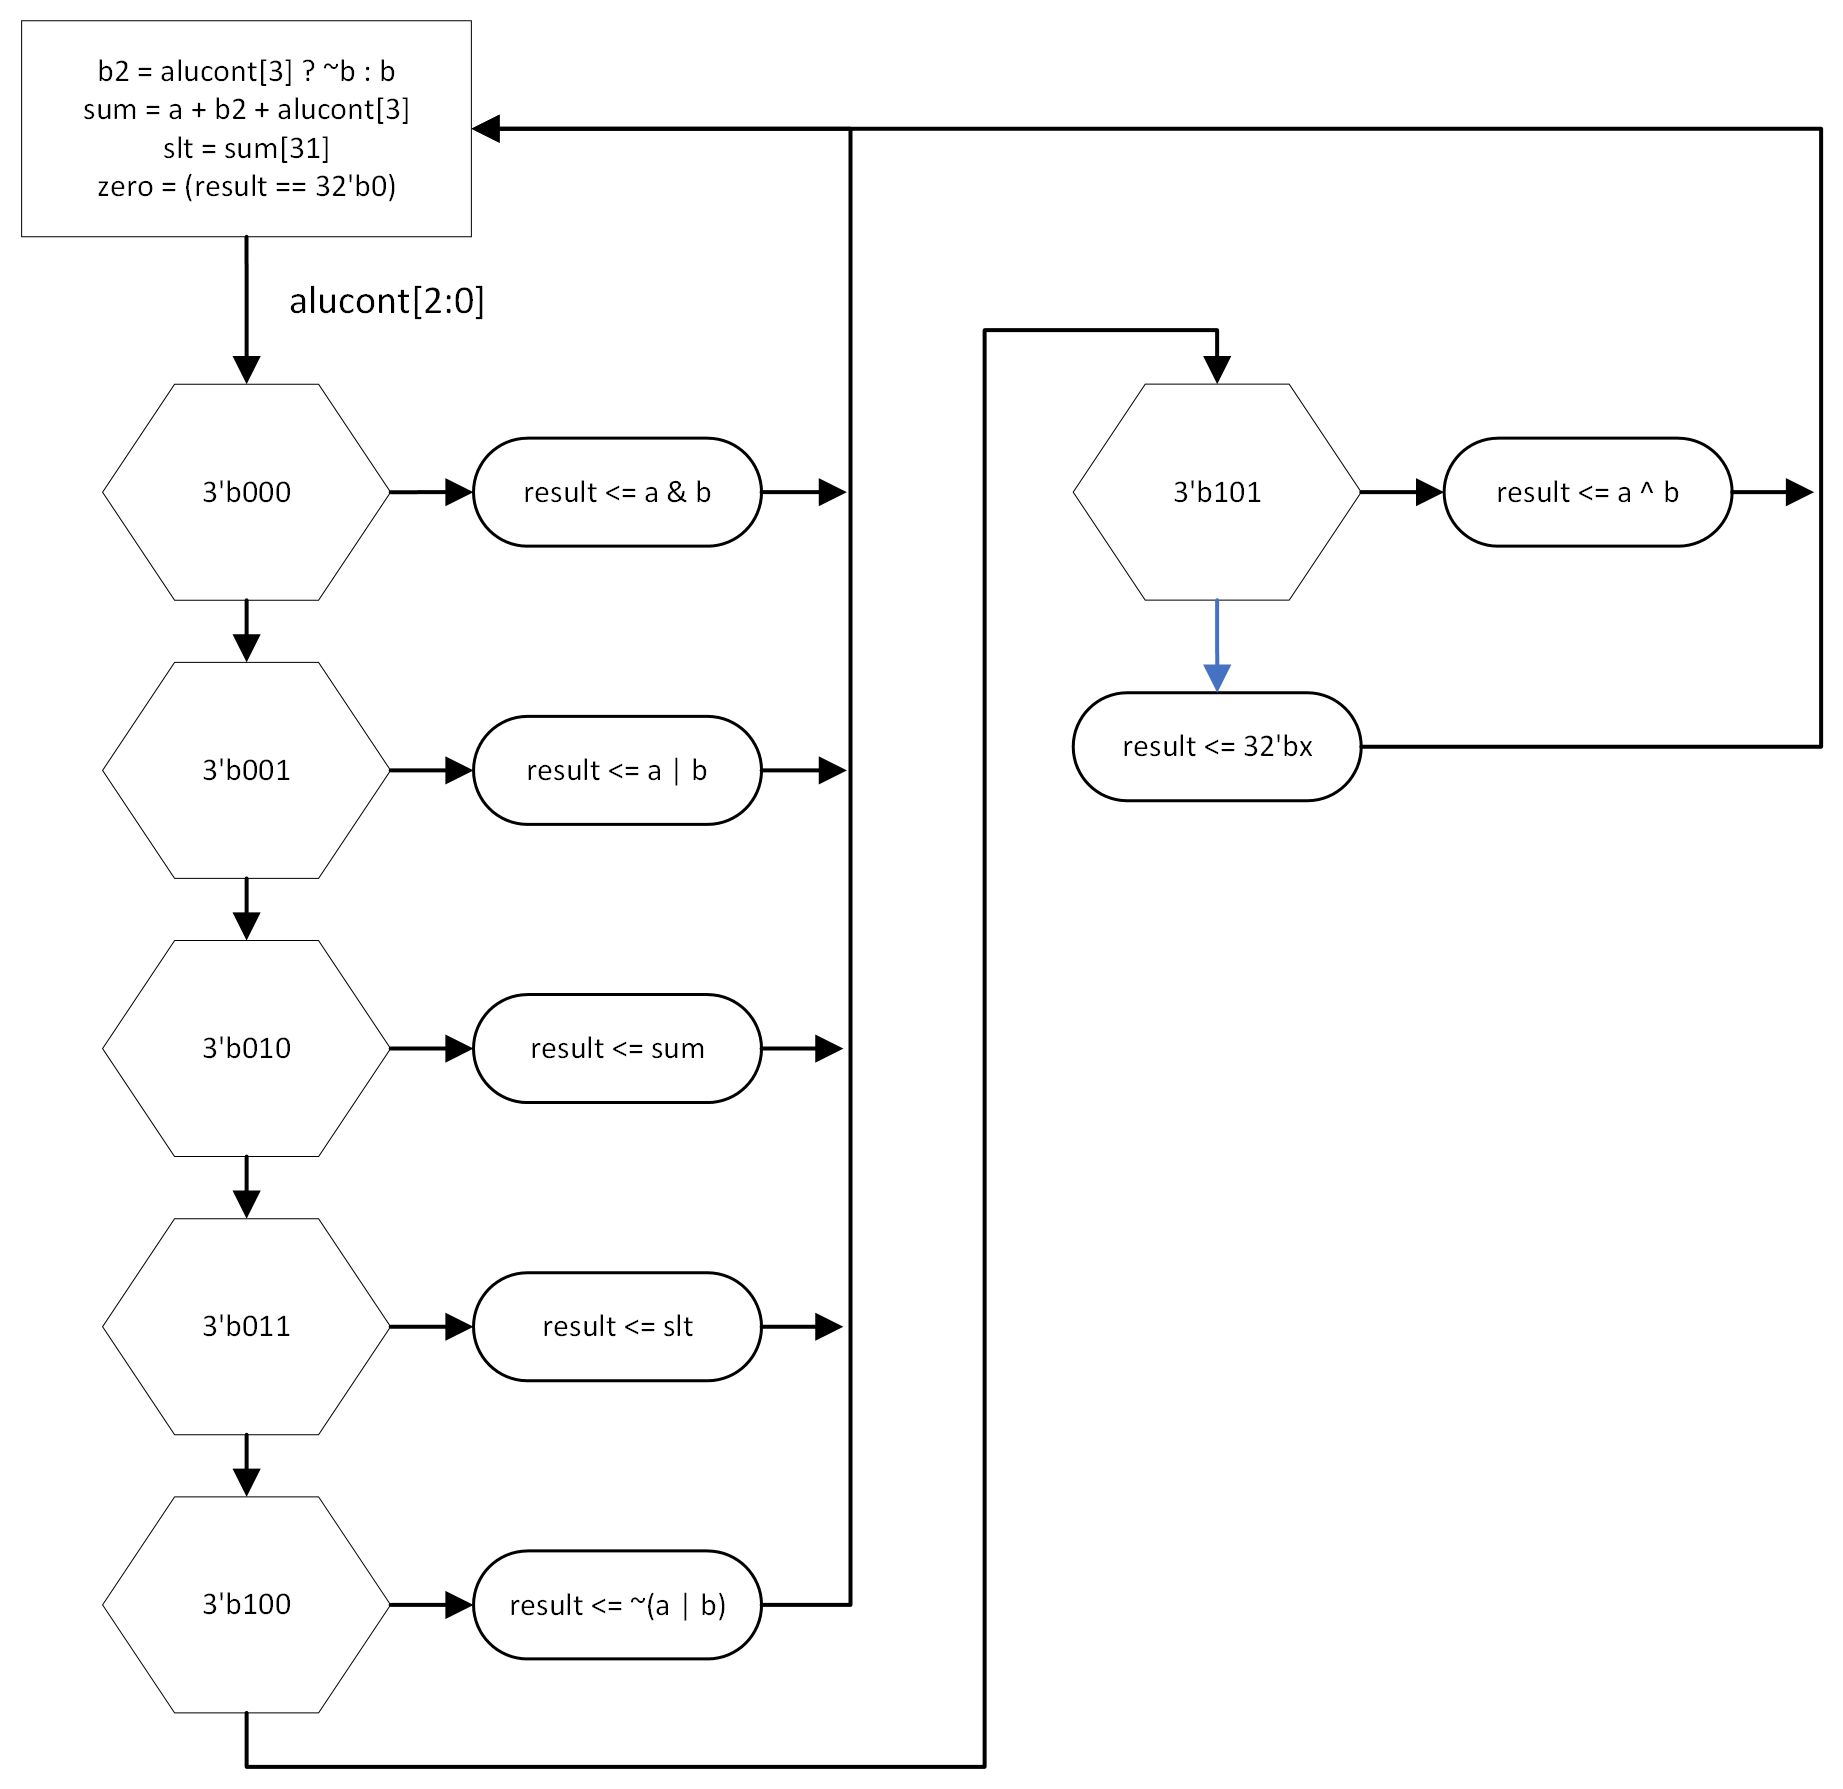
\includegraphics[width=\textwidth]{alu_asm}
   \caption{ASM chart for the ALU module.}
   \label{fig:alu_asm}
\end{figure}

\begin{figure}[htbp]
   \centering
   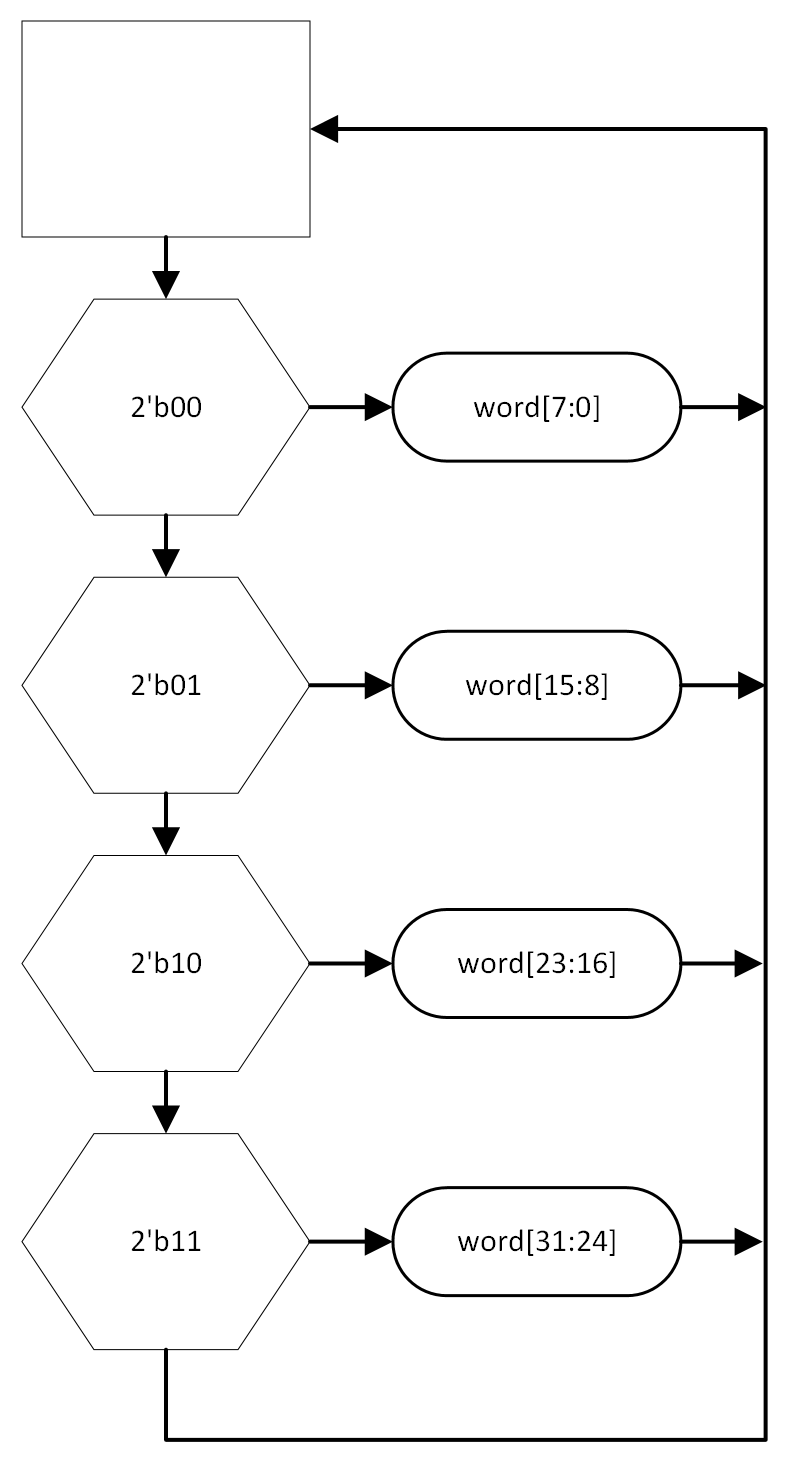
\includegraphics[width=0.4\textwidth]{mux4_asm}
   \caption{ASM chart for the four inputs multiplexer module.}
   \label{fig:mux4_asm}
\end{figure}

\begin{figure}[htbp]
   \centering
   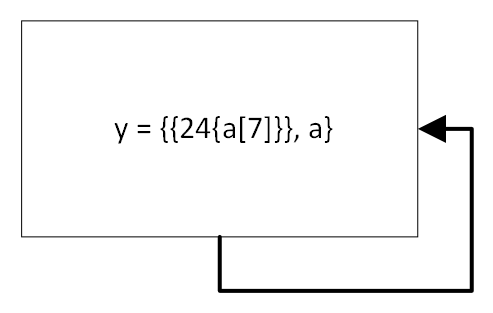
\includegraphics[width=0.4\textwidth]{sign_ext_asm}
   \caption{ASM chart for the sign extension module.}
   \label{fig:sign_ext_asm}
\end{figure}

\begin{figure}[htbp]
   \centering
   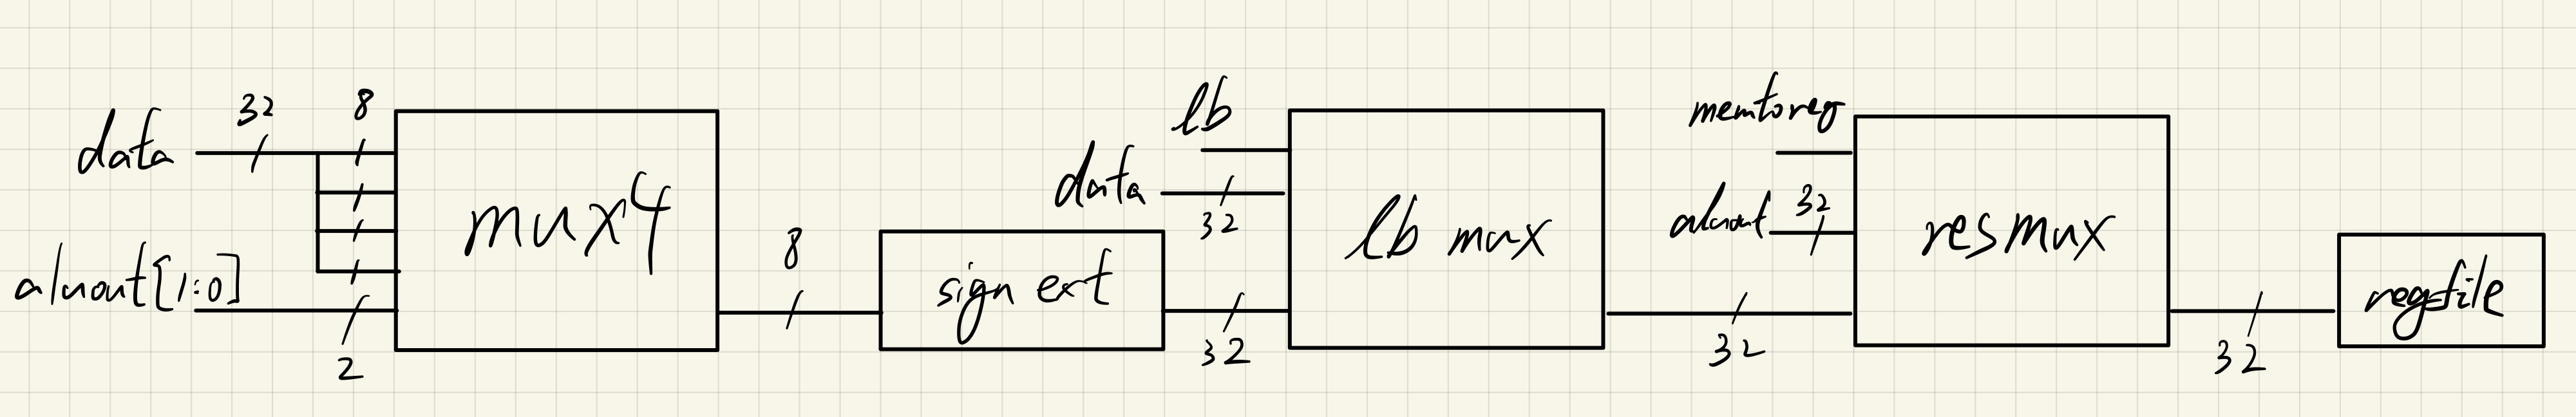
\includegraphics[width=\textwidth]{lb_block}
   \caption{Block diagram of the \textit{lb} implementation design.}
   \label{fig:lb_block}
\end{figure}

\newpage

To add \textit{nor}, \textit{xori}, and \textit{lb} to the existing design, the following modifications were made.

\begin{minted}[
   fontsize=\footnotesize,
   linenos,
   breaklines,
]{udiff}
--- MIPS_System_Students\MIPS_CPU\mipsparts.v	2013-02-08 11:49:24.000000000 +0100
+++ MIPS_System_Students\MIPS_CPU\mipsparts.v	2023-04-20 16:22:16.000000000 +0100
@@ -18,28 +18,31 @@
   assign rd1 = (ra1 != 0) ? rf[ra1] : 0;
   assign rd2 = (ra2 != 0) ? rf[ra2] : 0;
 endmodule
 
 
 module alu(input      [31:0] a, b, 
-           input      [2:0]  alucont, 
+           input      [3:0]  alucont, 
            output reg [31:0] result,
            output            zero);
 
   wire [31:0] b2, sum, slt;
 
-  assign b2 = alucont[2] ? ~b:b; 
-  assign sum = a + b2 + alucont[2];
+  assign b2 = alucont[3] ? ~b : b; 
+  assign sum = a + b2 + alucont[3];
   assign slt = sum[31];
 
   always@(*)
-    case(alucont[1:0])
-      2'b00: result <= a & b;
-      2'b01: result <= a | b;
-      2'b10: result <= sum;
-      2'b11: result <= slt;
+    case(alucont[2:0])
+      3'b000: result <= a & b;
+      3'b001: result <= a | b;
+      3'b010: result <= sum;
+      3'b011: result <= slt;
+      3'b100: result <= ~(a | b); // NOR
+      3'b101: result <= a ^ b; // XOR
+      default: result <= 32'bx; // FIXME: I don't know whether this is a sensible default
     endcase
 
   assign zero = (result == 32'b0);
 
 endmodule
 
@@ -121,6 +124,48 @@
               input              s, 
               output [WIDTH-1:0] y);
 
   assign y = s ? d1 : d0; 
 
 endmodule
+
+
+
+module mux4 #(
+    parameter WIDTH = 8
+)(
+    input  [WIDTH-1:0] d0, d1, d2, d3,
+    input  [1:0] s,
+    output reg [WIDTH-1:0] y
+);
+
+always @(d0, d1, d2, d3, s)
+    case (s)
+       2'b00: y <= d0;
+       2'b01: y <= d1;
+       2'b10: y <= d2;
+       2'b11: y <= d3;
+    endcase
+
+endmodule
+
+
+
+module sign_ext(
+    input  [7:0] a,
+    output [31:0] y
+);
+
+    assign y = {{24{a[7]}}, a};
+
+endmodule
+
+
+
+module zero_ext(
+    input  [7:0] a,
+    output [31:0] y
+);
+
+    assign y = {24'b0, a};
+
+endmodule
\end{minted}

\begin{minted}[
   fontsize=\footnotesize,
   linenos,
   breaklines,
]{udiff}
--- MIPS_System_Students\MIPS_CPU\mips.v	2013-02-08 11:48:52.000000000 +0100
+++ MIPS_System_Students\MIPS_CPU\mips.v	2023-04-20 16:23:12.000000000 +0100
@@ -19,14 +19,14 @@
             output [31:0] memaddr,
             output [31:0] memwritedata,
             input  [31:0] memreaddata);
 
   wire        signext, shiftl16, memtoreg, branch;
   wire        pcsrc, zero;
-  wire        alusrc, regdst, regwrite, jump;
-  wire [2:0]  alucontrol;
+  wire        alusrc, regdst, regwrite, jump, lb;
+  wire [3:0]  alucontrol;
 
   // Instantiate Controller
   controller c(.op         (instr[31:26]), 
                .funct      (instr[5:0]), 
                .zero       (zero),
                .signext    (signext), 
@@ -35,12 +35,13 @@
                .memwrite   (memwrite), 
                .pcsrc      (pcsrc),
                .alusrc     (alusrc), 
                .regdst     (regdst), 
                .regwrite   (regwrite), 
                .jump       (jump),
+               .lb         (lb),
                .alucontrol (alucontrol));
 
   // Instantiate Datapath
   datapath dp( .clk        (clk), 
                .reset      (reset), 
                .signext    (signext), 
@@ -48,12 +49,13 @@
                .memtoreg   (memtoreg), 
                .pcsrc      (pcsrc),
                .alusrc     (alusrc), 
                .regdst     (regdst), 
                .regwrite   (regwrite), 
                .jump       (jump),
+               .lb         (lb),
                .alucontrol (alucontrol),
                .zero       (zero), 
                .pc         (pc), 
                .instr      (instr),
                .aluout     (memaddr), 
                .writedata  (memwritedata), 
@@ -67,27 +69,29 @@
                   output       signext,
                   output       shiftl16,
                   output       memtoreg, memwrite,
                   output       pcsrc, alusrc,
                   output       regdst, regwrite,
                   output       jump,
-                  output [2:0] alucontrol);
+                  output       lb,
+                  output [3:0] alucontrol);
 
-  wire [1:0] aluop;
+  wire [2:0] aluop;
   wire       branch;
 
   maindec md( .op    (op), 
               .signext   (signext), 
               .shiftl16  (shiftl16), 
               .memtoreg  (memtoreg), 
               .memwrite  (memwrite), 
               .branch    (branch),
               .alusrc    (alusrc), 
               .regdst    (regdst), 
               .regwrite  (regwrite), 
               .jump      (jump),
+              .lb        (lb),
               .aluop     (aluop));
 
   aludec  ad( .funct      (funct), 
               .aluop      (aluop), 
               .alucontrol (alucontrol));
 
@@ -100,77 +104,84 @@
                output       signext,
                output       shiftl16,
                output       memtoreg, memwrite,
                output       branch, alusrc,
                output       regdst, regwrite,
                output       jump,
-               output [1:0] aluop);
+               output       lb,
+               output [2:0] aluop);
 
-  reg [10:0] controls;
+  reg [12:0] controls;
 
-  assign {signext, shiftl16, regwrite, regdst, 
-          alusrc, branch, memwrite,
-          memtoreg, jump, aluop} = controls;
+  assign {signext, shiftl16, regwrite, regdst, alusrc, branch, memwrite, memtoreg, jump, lb, aluop} = controls;
 
   always @(*)
-    case(op)
-      6'b000000: controls <= 11'b00110000011; // Rtype
-      6'b100011: controls <= 11'b10101001000; // LW
-      6'b101011: controls <= 11'b10001010000; // SW
-      6'b000100: controls <= 11'b10000100001; // BEQ
+    case(op)                                    // aluop
+      6'b000000: controls <= 13'b0_0_1_1_0_0_0_0_0_0_111; // Rtype
+      6'b100011: controls <= 13'b1_0_1_0_1_0_0_1_0_0_000; // LW
+      6'b100000: controls <= 13'b1_0_1_0_1_0_0_1_0_1_000; // LB  signext regwrite alusrc memtoreg
+      6'b101011: controls <= 13'b1_0_0_0_1_0_1_0_0_0_000; // SW
+      6'b000100: controls <= 13'b1_0_0_0_0_1_0_0_0_0_001; // BEQ
       6'b001000, 
-      6'b001001: controls <= 11'b10101000000; // ADDI, ADDIU: only difference is exception
-      6'b001101: controls <= 11'b00101000010; // ORI
-      6'b001111: controls <= 11'b01101000000; // LUI
-      6'b000010: controls <= 11'b00000000100; // J
-      default:   controls <= 11'bxxxxxxxxxxx; // ???
+      6'b001001: controls <= 13'b1_0_1_0_1_0_0_0_0_0_000; // ADDI, ADDIU: only difference is exception
+      6'b001101: controls <= 13'b0_0_1_0_1_0_0_0_0_0_010; // ORI
+      6'b001110: controls <= 13'b0_0_1_0_1_0_0_0_0_0_011; // XORI
+      6'b001111: controls <= 13'b0_1_1_0_1_0_0_0_0_0_000; // LUI
+      6'b000010: controls <= 13'b0_0_0_0_0_0_0_0_1_0_000; // J
+      default:   controls <= 13'bx_x_x_x_x_x_x_x_x_x_xxx; // ???
     endcase
 
 endmodule
 
 module aludec(input      [5:0] funct,
-              input      [1:0] aluop,
-              output reg [2:0] alucontrol);
+              input      [2:0] aluop,
+              output reg [3:0] alucontrol);
 
   always @(*)
     case(aluop)
-      2'b00: alucontrol <= 3'b010;  // add
-      2'b01: alucontrol <= 3'b110;  // sub
-      2'b10: alucontrol <= 3'b001;  // or
-      default: case(funct)          // RTYPE
+      3'b000: alucontrol <= 4'b0_010;  // add
+      3'b001: alucontrol <= 4'b1_010;  // sub
+      3'b010: alucontrol <= 4'b0_001;  // or
+      3'b011: alucontrol <= 4'b0_101;  // xori
+      default: case(funct) // RTYPE
           6'b100000,
-          6'b100001: alucontrol <= 3'b010; // ADD, ADDU: only difference is exception
+          6'b100001: alucontrol <= 4'b0_010; // ADD, ADDU: only difference is exception
           6'b100010,
-          6'b100011: alucontrol <= 3'b110; // SUB, SUBU: only difference is exception
-          6'b100100: alucontrol <= 3'b000; // AND
-          6'b100101: alucontrol <= 3'b001; // OR
-          6'b101010: alucontrol <= 3'b111; // SLT
-          default:   alucontrol <= 3'bxxx; // ???
-        endcase
+          6'b100011: alucontrol <= 4'b1_010; // SUB, SUBU: only difference is exception
+          6'b100100: alucontrol <= 4'b0_000; // AND
+          6'b100101: alucontrol <= 4'b0_001; // OR
+          6'b101010: alucontrol <= 4'b1_011; // SLT
+          6'b100111: alucontrol <= 4'b0_100; // NOR
+          default:   alucontrol <= 4'bx_xxx; // ???
+       endcase
     endcase
 endmodule
 
 module datapath(input         clk, reset,
                 input         signext,
                 input         shiftl16,
                 input         memtoreg, pcsrc,
                 input         alusrc, regdst,
                 input         regwrite, jump,
-                input  [2:0]  alucontrol,
+                input         lb,
+                input  [3:0]  alucontrol,
                 output        zero,
                 output [31:0] pc,
                 input  [31:0] instr,
                 output [31:0] aluout, writedata,
                 input  [31:0] readdata);
 
   wire [4:0]  writereg;
   wire [31:0] pcnext, pcnextbr, pcplus4, pcbranch;
   wire [31:0] signimm, signimmsh, shiftedimm;
   wire [31:0] srca, srcb;
   wire [31:0] result;
   wire        shift;
+  wire [31:0] lbres;
+  wire [31:0] seres;
+  wire [7:0] byteres;
 
   // next PC logic
   flopr #(32) pcreg (.clk   (clk), 
                      .reset (reset), 
                      .d     (pcnext), 
                      .q     (pc));
@@ -207,32 +218,65 @@
                     .rd2     (writedata));
 
   mux2 #(5)   wrmux(.d0  (instr[20:16]), 
                     .d1  (instr[15:11]), 
                     .s   (regdst), 
                     .y   (writereg));
 
+  mux4 bytemux(
+      .d0 (readdata[7:0]), 
+      .d1 (readdata[15:8]), 
+      .d2 (readdata[23:16]), 
+      .d3 (readdata[31:24]), 
+      .s  (aluout[1:0]), 
+      .y  (byteres)
+  );
+
+  sign_ext  se(
+      .a (byteres),
+      .y (seres)
+  );
+
+  mux2 #(32)  lbmux(
+      .d0 (readdata), 
+      .d1 (seres), 
+      .s  (lb), 
+      .y  (lbres)
+  );
+
-  mux2 #(32)  resmux(.d0 (aluout), 
-                     .d1 (readdata), 
-                     .s  (memtoreg), 
-                     .y  (result));
+  mux2 #(32)  resmux(
+      .d0 (aluout), 
+      .d1 (lbres), 
+      .s  (memtoreg), 
+      .y  (result)
+  );
 
-  sign_zero_ext  sze(.a       (instr[15:0]), 
+  sign_zero_ext  sze(.a       (instr[15:0]),  // filled the left 32 bits with the sign bit
                     .signext (signext),
                     .y       (signimm[31:0]));
 
   shift_left_16 sl16(.a         (signimm[31:0]), 
                      .shiftl16  (shiftl16),
                      .y         (shiftedimm[31:0]));
 
   // ALU logic
-  mux2 #(32)  srcbmux(.d0 (writedata), 
-                      .d1 (shiftedimm[31:0]), 
-                      .s  (alusrc), 
-                      .y  (srcb));
+  mux2 #(32)  srcbmux(.d0 (writedata),  // data from a reg
+                      .d1 (shiftedimm[31:0]), // stands for immediate/offset
+                      .s  (alusrc),  // if `alusrc` is 1, select `d1`
+                      .y  (srcb));  // d0 or d1
 
   alu         alu( .a       (srca), 
                    .b       (srcb), 
                    .alucont (alucontrol),
                    .result  (aluout), 
                    .zero    (zero));
 endmodule
\end{minted}

The principle of the \textit{lb} implementation is complex. A typical form of the \textit{lb} instruction is
\begin{minted}[
   fontsize=\footnotesize,
   breaklines,
]{mips}
lb rd, imm(addr)
\end{minted}
ALU outputs \textit{addr} + \textit{imm} as the data address to the data memory for reading a data. On the other hand, the data memory ignores the two least significant value of the input data address:
\begin{minted}[
   fontsize=\footnotesize,
   breaklines,
]{verilog}
ram2port_inst_data Inst_Data_Mem (
   .address_a   (inst_addr[12:2]),
   .address_b   (data_addr[12:2]),
\end{minted}
Thus, we can use the last two bits of the immediate value, which is effectively the last two bits of the ALU output provided that the last two bits of the \textit{addr} are both zero (remember \textit{aluout} = \textit{addr} + \textit{imm}), for selecting the byte of the data stored at the address \textit{addr}.

\subsection{Testing}

Below is the test code for \textit{nor}, \textit{xori}, and \textit{lb}.

\begin{minted}[
   fontsize=\footnotesize,
   linenos,
   breaklines,
]{MIPS}
### nor

# Test data 0xFF00 F0F0
lui $t0, 0xFF00
ori $t0, $t0, 0xF0F0

nor $t1, $t0, $zero  # Invert all bits; expect 0x00FF 0F0F



### xori

# Test data 0x7B41 92C0
lui $t0, 0x7B41
ori $t0, $t0, 0x92C0

xori $t1, $t0, 0x5730  # expect GPR 1 contains 0x7B41 C5F0



### lb

# Store test data 0xAABB CCDD to GPR 9
lui $t9, 0x0000
addiu $t9, $t9, 0x0200
lui $t0, 0xAABB
ori $t0, $t0, 0xCCDD
sw $t0, 0x0000($t9)

lb $t1, 0x0000($t9)
lb $t2, 0x0001($t9)
lb $t3, 0x0002($t9)
lb $t4, 0x0003($t9)
\end{minted}

Figure \ref{fig:part_b} is the overview of the test results for Part B. Figure \ref{fig:nor}, \ref{fig:xori}, and \ref{fig:lb} are the test result for \textit{nor}, \textit{xori}, and \textit{lb}, respectively.

\begin{figure}[htbp]
   \centering
   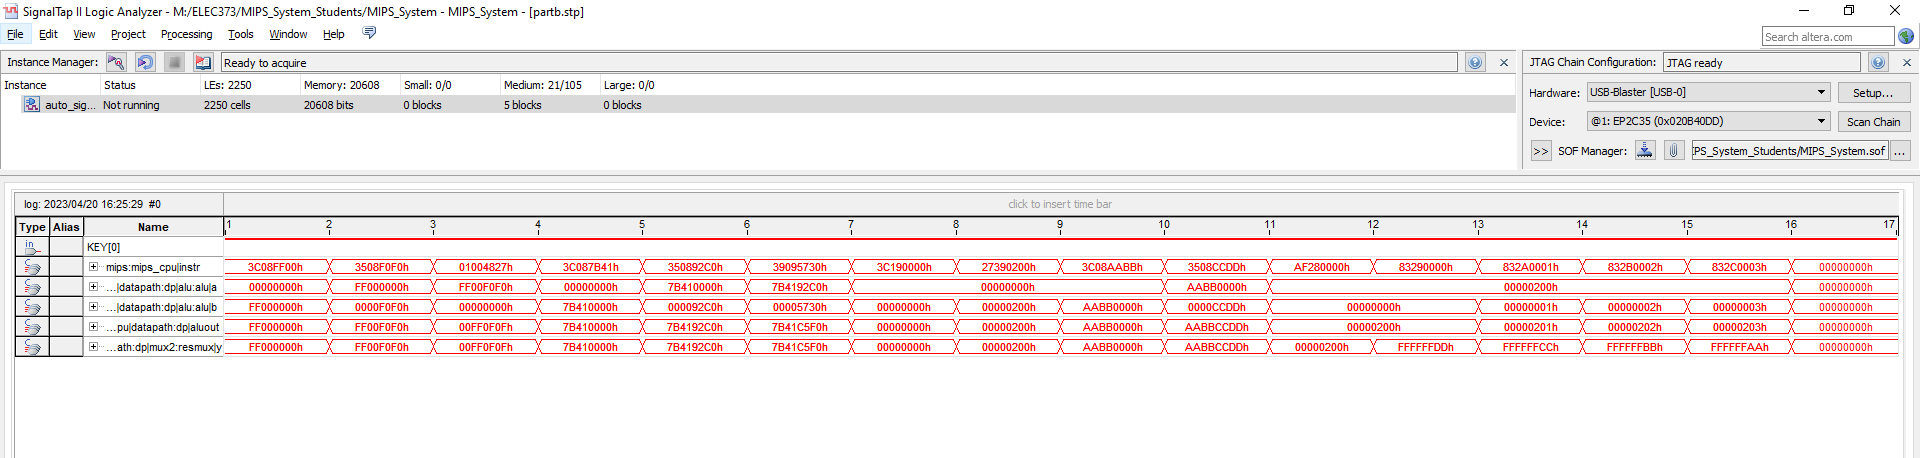
\includegraphics[width=\textwidth]{part_b}
   \caption{Test results of Part B visualised by SignalTap.}
   \label{fig:part_b}
\end{figure}

\begin{figure}[htbp]
   \centering
   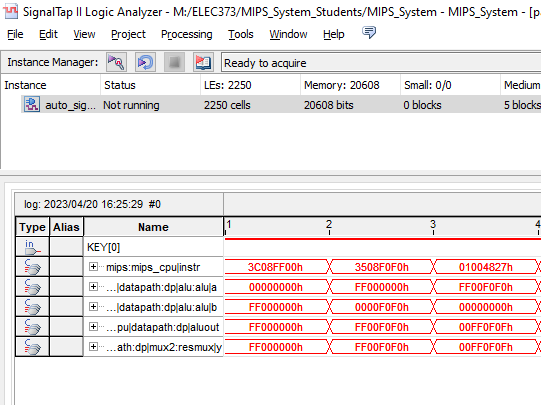
\includegraphics[width=\textwidth]{part_b_1}
   \caption{Expected test result of \textit{nor}.}
   \label{fig:nor}
\end{figure}

\begin{figure}[htbp]
   \centering
   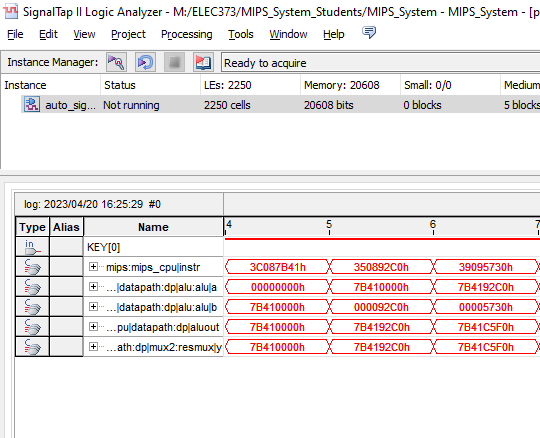
\includegraphics[width=\textwidth]{part_b_2}
   \caption{Expected test result of \textit{xori}.}
   \label{fig:xori}
\end{figure}

\begin{figure}[htbp]
   \centering
   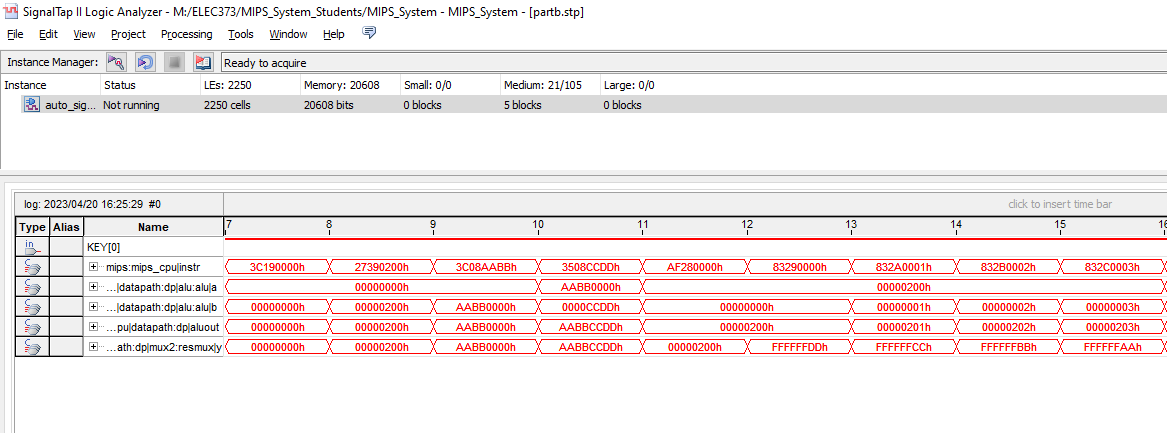
\includegraphics[width=\textwidth]{part_b_3}
   \caption{Expected test result of \textit{lb}.}
   \label{fig:lb}
\end{figure}

\newpage
\subsubsection{Code coverage}

High test coverage could help to ensure modifications don't affect other functionalities. There are numerous coverage criteria such as function coverage and condition coverage. For this task, we want to have high function coverage to ensure the modification doesn't affect the other instruction implementation. The test code below covers all the implemented instructions.

\begin{minted}[
   fontsize=\footnotesize,
   linenos,
   breaklines,
]{MIPS}
# lui ori
lui $s0, 0x0000
ori $s0, $s0, 0x0200

# sw lw

lui $s1, 0xAABB
ori $s1, $s1, 0xCCDD

sw $s1, 0x0000($s0)
lw $t0, 0x0000($s0)

# lb

lb $t0, 0x0000($s0)
lb $t0, 0x0001($s0)
lb $t0, 0x0002($s0)
lb $t0, 0x0003($s0)

# nor

lui $s1, 0xFF00
ori $s1, $s1, 0xF0F0  # Test data 0xFF00 F0F0

nor $t0, $s1, $zero  # Invert all bits; expect 0x00FF 0F0F

# xori

lui $s1, 0x7B41
ori $s1, $s1, 0x92C0  # Test data 0x7B41 92C0

xori $t0, $s1, 0x5730  # Expect 0x7B41 C5F0

# and or

lui $s1, 0xF0F0
ori $s1, $s1, 0xF0F0

lui $s2, 0x0F0F
ori $s2, $s2, 0x0F0F

and $t0, $s1, $s2  # Expect 0x0000 0000
or $t0, $s1, $s2   # Expect 0xFFFF FFFF

# slt

lui $s1, 0x6666
ori $s1, $s1, 0x6666

lui $s2, 0x7777
ori $s2, $s2, 0x7777

slt $t0, $s1, $s2  # Expect being set to 1

# addi, addiu, add, addu

lui $s1, 0x7FFF
ori $s1, $s1, 0xFFFF  # Max positive int in 2's complement

addi $t0, $s1, 0x0001  # Expect 0x8000 0000 with overflow
addiu $t0, $s1, 0x0001  # Expect 0x8000 0000 without overflow

lui $s2, 0x0000
ori $s2, $s2, 0x0001

add $t0, $s1, $s2  # Expect 0x8000 0000 with overflow
addu $t0, $s1, $s2  # Expect 0x8000 0000 without overflow

# sub, subu

lui $s1, 0x8000
ori $s1, $s1, 0x0000  # Min negative int in 2's complement

lui $s2, 0x0000
ori $s2, $s2, 0x0001

sub $t0, $s1, $s2  # Expect 0x7FFF FFFF with overflow
subu $t0, $s1, $s2  # Expect 0x7FFF FFFF without overflow

# beq

lui $s1, 0x6666
ori $s1, $s1, 0x6666  # Min negative int in 2's complement

lui $s2, 0x6666
ori $s2, $s2, 0x6666

beq $s1, $s2, GOTO
add $t0, $t0, $t0  # Random instr
GOTO:

# j

j End
add $t0, $t0, $t0  # Random instr
End:
\end{minted}

\begin{figure}[htbp]
   \centering
   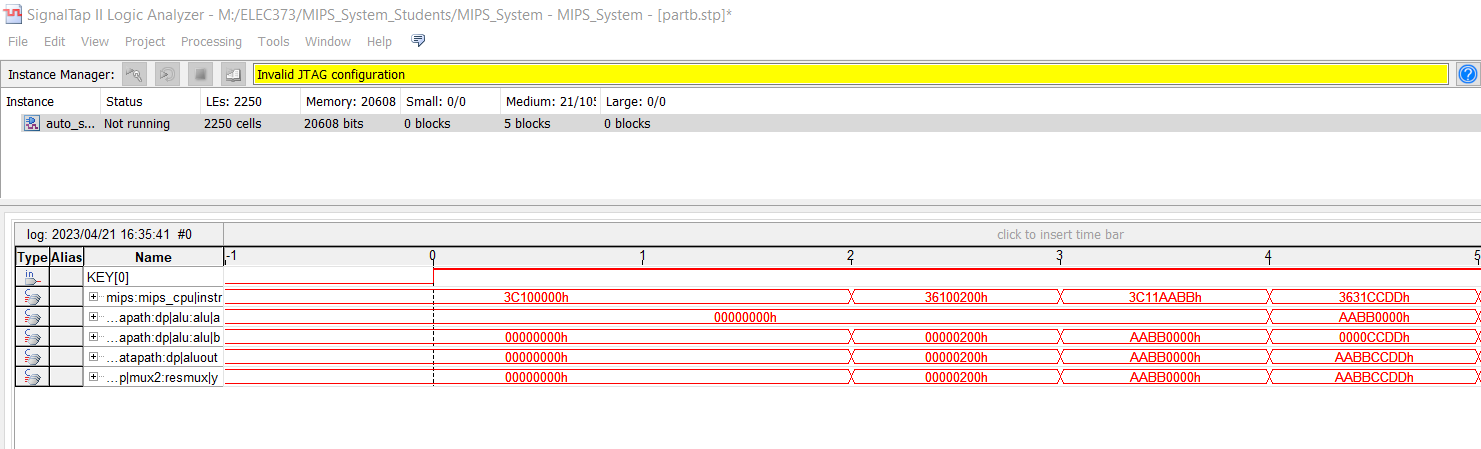
\includegraphics[width=\textwidth]{lui_ori_sw_lw}
   \caption{Store 0xAABB CCDD to address 0x000 0200 with \textit{lui}, \textit{ori}, \textit{sw}, and \textit{lw}.}
\end{figure}

\begin{figure}[htbp]
   \centering
   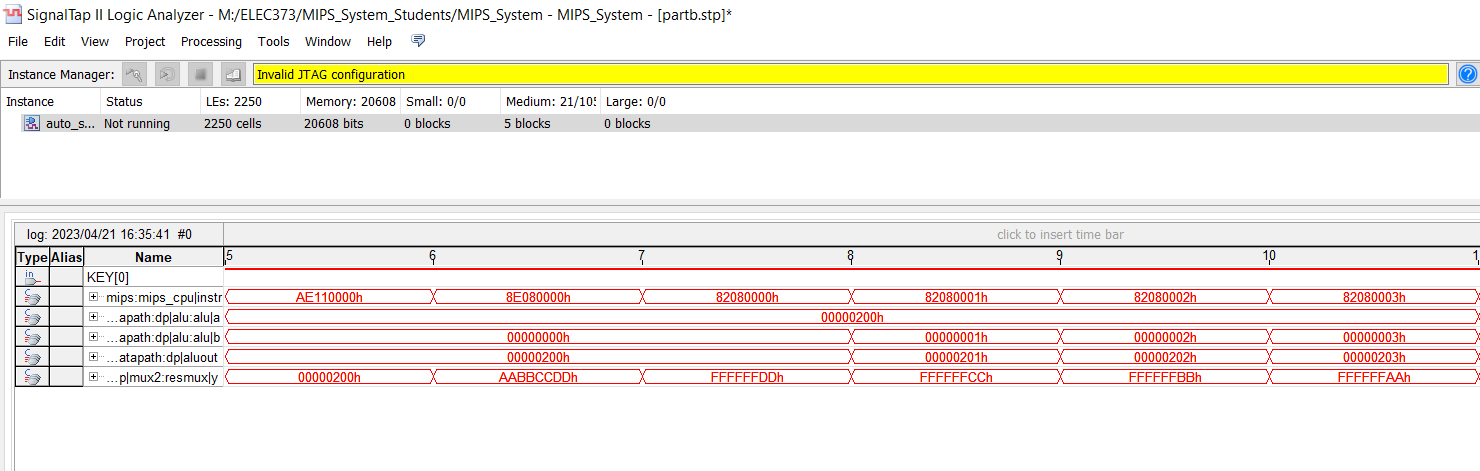
\includegraphics[width=\textwidth]{lb}
   \caption{Pick byte DD, CC, BB, and AA from 0xAABB CCDD with sign extension.}
\end{figure}

\begin{figure}[htbp]
   \centering
   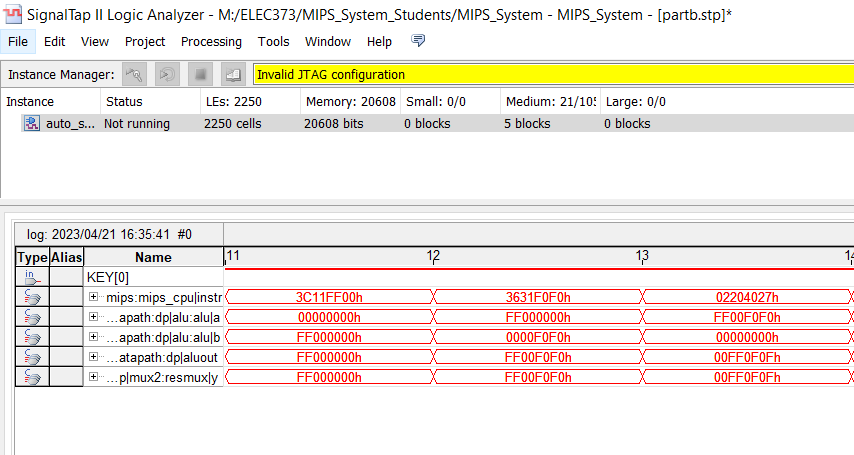
\includegraphics[width=\textwidth]{nor}
   \caption{Invert all bit of 0xFF00 F0F0 to 00FF 0F0F by \textit{nor} it with zeros.}
\end{figure}

\begin{figure}[htbp]
   \centering
   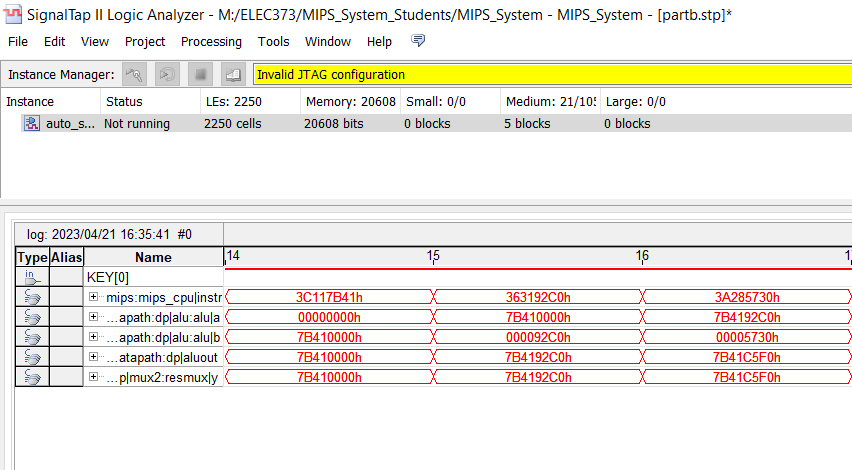
\includegraphics[width=\textwidth]{xori}
   \caption{0x7B41 92C0 \textit{xori} 0x0000 5730 yields 0x7B41 C5F0.}
\end{figure}

\begin{figure}[htbp]
   \centering
   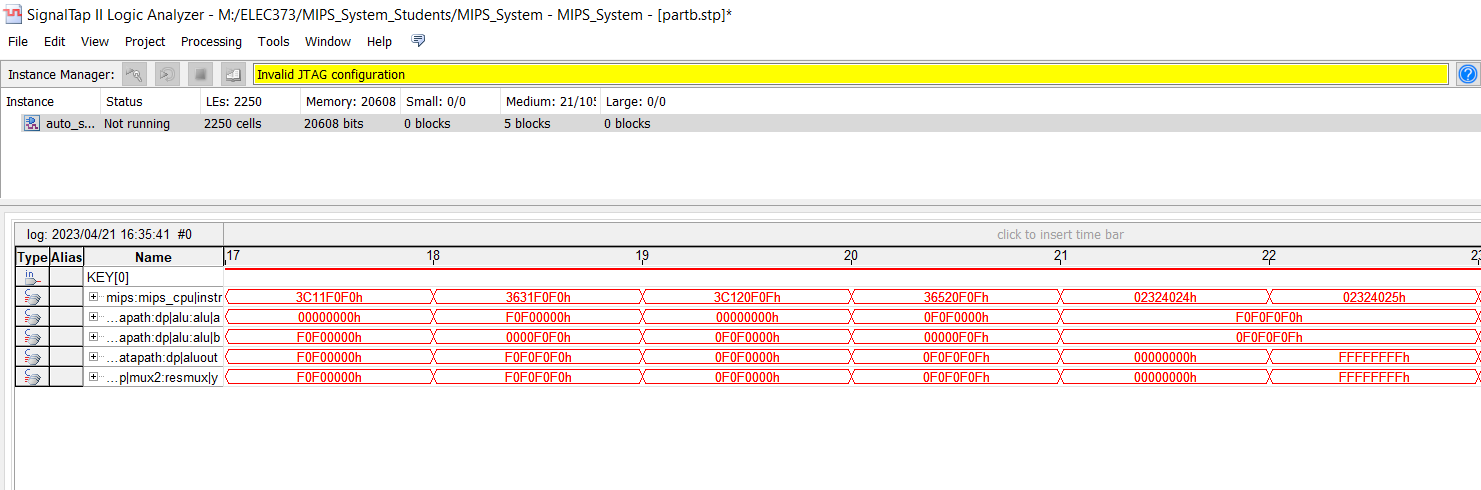
\includegraphics[width=\textwidth]{and_or}
   \caption{0xF0F0 F0F0 \textit{and} 0x0F0F 0F0F yields 0x0000 0000, \textit{or} yields 0xFFFF FFFF.}
\end{figure}

\begin{figure}[htbp]
   \centering
   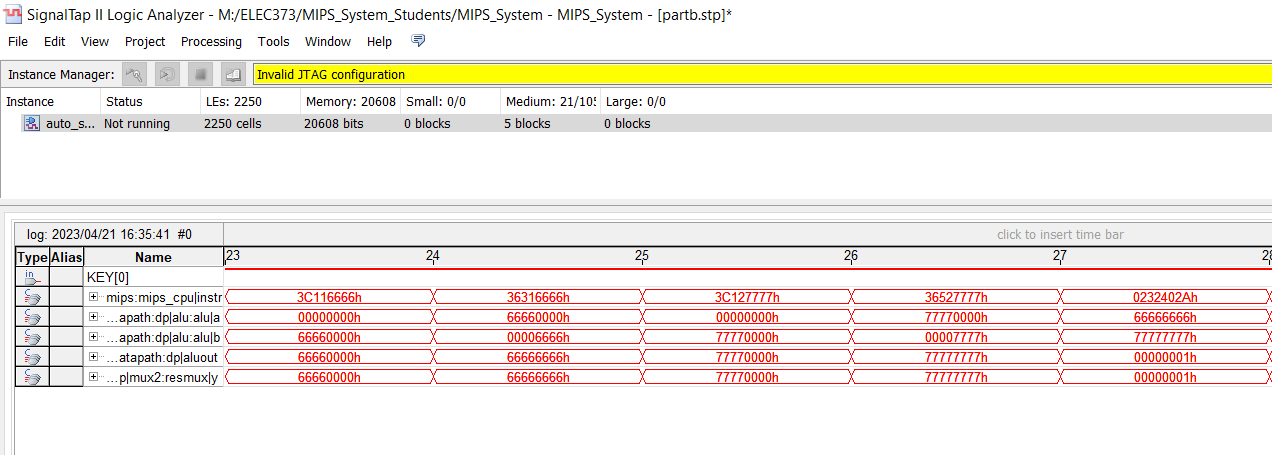
\includegraphics[width=\textwidth]{stl}
   \caption{Set 1 because 0x6666 6666 less than 0x7777 7777.}
\end{figure}

\begin{figure}[htbp]
   \centering
   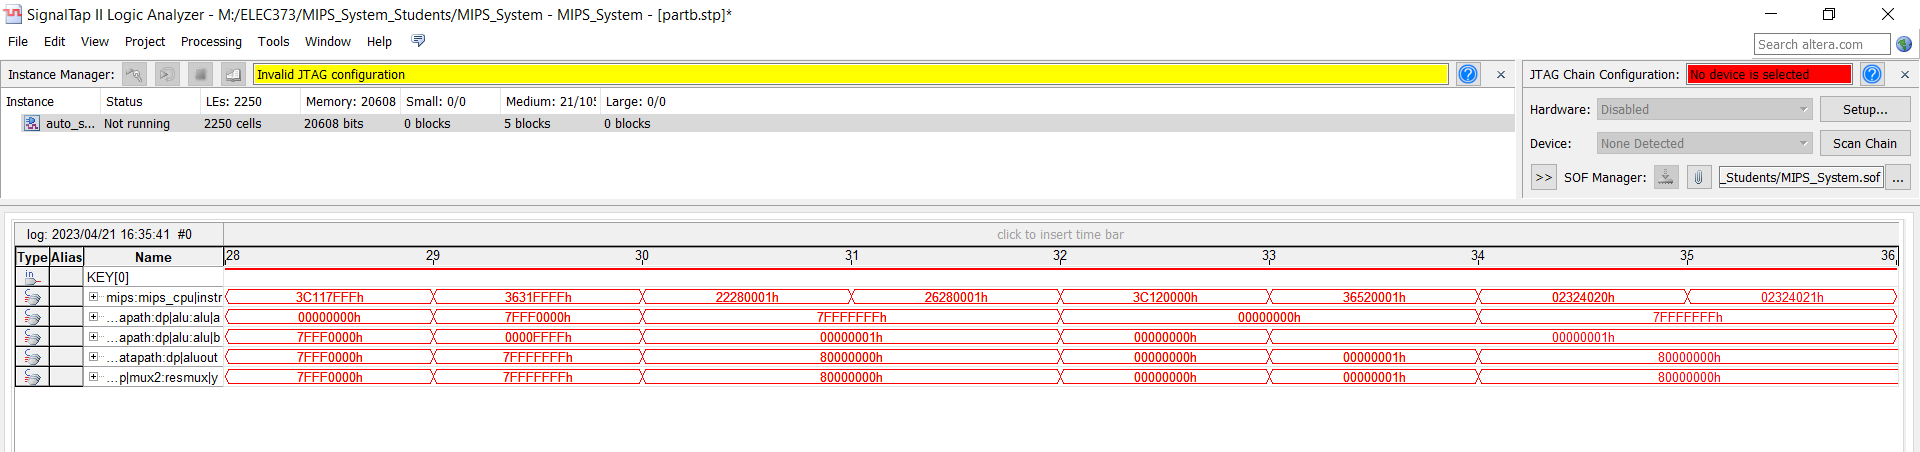
\includegraphics[width=\textwidth]{addi_addiu_add_addu}
   \caption{Expected test result of \textit{addi}, \textit{addiu}, \textit{add}, and \textit{addu}. The given MIPS implementation does not implement signalling overflow exception, so the overflow condition cannot be tested.}
\end{figure}

\begin{figure}[htbp]
   \centering
   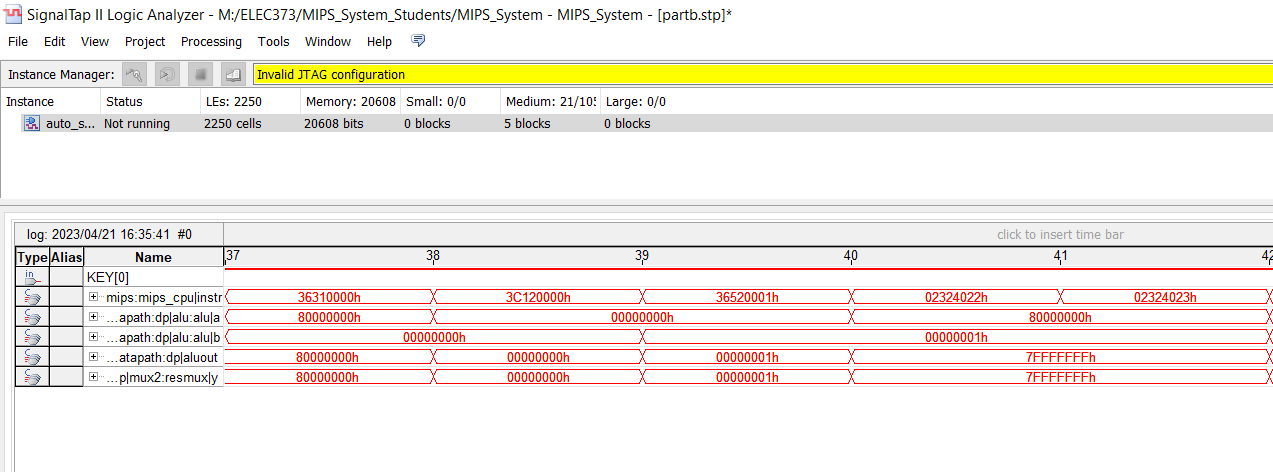
\includegraphics[width=\textwidth]{sub_subu}
   \caption{Expected test result of \textit{sub} and \textit{subu}. Again, the overflow condition cannot be tested.}
\end{figure}

\begin{figure}[htbp]
   \centering
   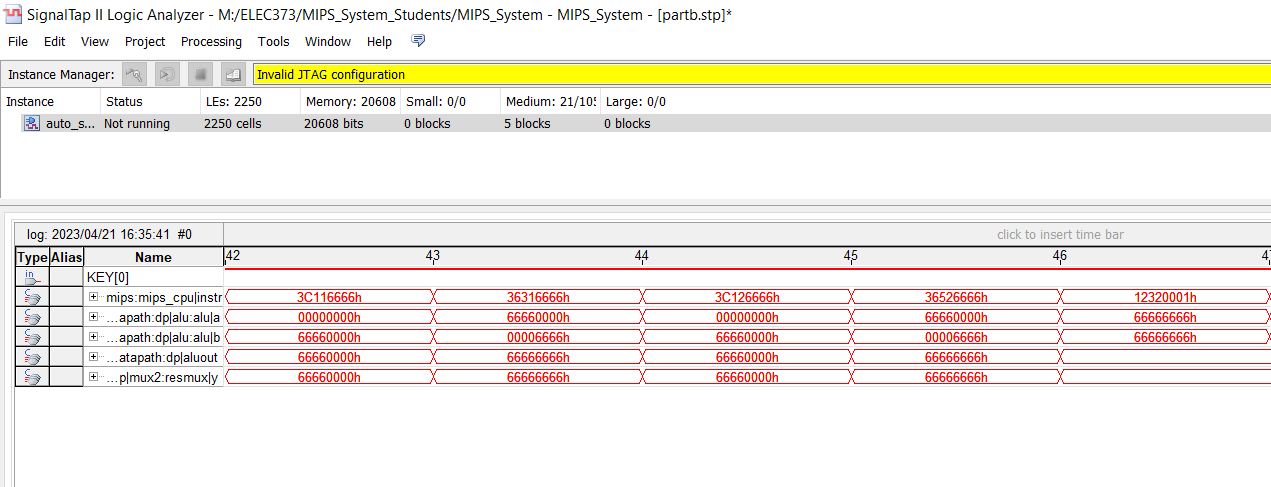
\includegraphics[width=\textwidth]{beq}
   \caption{Two values were equal, branching to a label was executed, and skipped an instruction.}
\end{figure}

\begin{figure}[htbp]
   \centering
   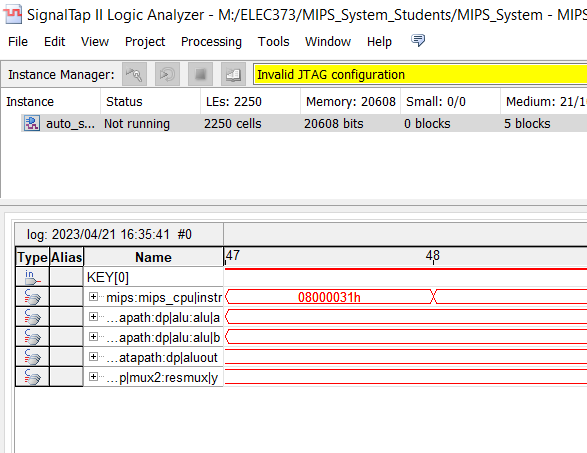
\includegraphics[width=\textwidth]{j}
   \caption{Jumped to a label and skipped an instruction.}
\end{figure}
